\documentclass[12pt]{article}

\usepackage[T1]{fontenc}
\usepackage[utf8]{inputenc}
\usepackage[italian]{babel}
\usepackage{fancyhdr}
\usepackage[margin=2cm]{geometry}
\usepackage{tocloft}
\usepackage{amsmath}
\usepackage{enumitem}
\usepackage{graphicx}
\usepackage{hyperref}

\renewcommand{\cftsecleader}{\cftdotfill{\cftdotsep}}
\renewcommand{\thesection}{\arabic{section}.}
\renewcommand{\thesubsection}{\arabic{section}.\arabic{subsection}}

\setlength{\headheight}{15pt}

\pagestyle{fancy}
\renewcommand{\footrulewidth}{0.4pt}
\lhead{\bfseries Requisiti di sistema}
\chead{}
\rhead{}
\lfoot{}
\cfoot{}
\rfoot{\thepage}

\begin{document}
\tableofcontents

\pagebreak

\section{Prefazione}

\subsection{Version History}

\begin{itemize}
\item Versione 0.0 - 16/04/2019 : Definizione piano di test 
\item Versione 1.0 - 04/05/2019 : Esiti dei test
\end{itemize}

\pagebreak

\section{Descrizione del prodotto software}
Il software, sviluppato in linguaggio Java in ambiente di sviluppo Eclipse, è suddiviso nei $4$ packages descritti di seguito:
\begin{itemize}
\item \textbf{lr1package} - questo package contiene due degli output di ANTLR, strumento utilizzato per generare il compilatore, ossia \textit{PrototipoLR1Lexer.java} e \textit{PrototipoLR1Parser.java}; il terzo e ultimo file di output (\textit{PrototipoLR1.tokens} è invece situato all'esterno di questo package;
\item \textbf{main\_package} - questo package contiene il file \textit{Riconoscitore.java}, all'interno del quale è definito il metodo \textit{main} che permette l'effettiva esecuzione del programma;
\item \textbf{myPackage} - questo package contiene il file \textit{Environment.java}, all'interno del quale è definita la classe Environment, necessaria per il corretto funzionamento dei file output di ANTLR ed ereditata da un progetto di esempio;
\item \textbf{solver} - questo package contiene tutti i file che contengono definizioni di classi custom utilizzate per il processo di riconoscimento delle grammatiche e per rappresentare gli elementi costituenti delle grammatiche.
\end{itemize}
La versione oggetto di test è la 1.0, pubblicata sul branch \textit{master} della repository di Github del progetto (\url{https://github.com/d-presciani/progettoLFC}) in data 26/03/2019.
\pagebreak
\section{Funzionalità oggetto di test}
Le funzionalità sottoposte a test di unità saranno quelle definite nelle classi contenute all'interno del package \textit{solver}, essendo queste le classi scritte manualmente e quelle che consentono l'effettivo funzionamento del programma; si tralascia di effettuare test di unità sui restanti package in quanto generati automaticamente da ANTLR e difficilmente sottoponibili a test di tale granularità. \par
È previsto anche un test di sistema, fornendo al sistema diversi input, per verificare la corretta integrazione tra i vari componenti e, al contempo, il corretto funzionamento del programma nel suo complesso. \par
Oltre ai suddetti test, è prevista anche l'esecuzione di un'analisi statica del codice tramite i due plugin di Eclipse \textit{SpotBugs} e \textit{PMD}.
\subsection{Elenco delle funzionalità oggetto di test}
Di seguito vengono riportate le classi, con i relativi metodi, per cui saranno effettuati i test di unità.
\begin{itemize}
\item Stato
\begin{itemize}
\item private void aggiungiCompletamento(RegolaDiProduzione nuovaRdp, RegolaDiProduzione regolaPadre)
\item public void aggiungiCore(RegolaDiProduzione rdp)
\item public Stato()
\item public void espandiStato(LinkedList<Stato> listaStati, LinkedList<String> listaTransizioni)
\item public String toString()
\end{itemize}
\item RegolaDiProduzione
\begin{itemize}
\item public RegolaDiProduzione()
\item public RegolaDiProduzione(NonTerminale parSX, List<Carattere> parDX)
\item public RegolaDiProduzione(RegolaDiProduzione reg)
\item public void addSeguito(String s)
\item public void avanzaPuntino()
\item public void calcolaAnnullabilita()
\item public boolean equals(Object o)
\item public String toString()
\end{itemize}
\item NonTerminale
\begin{itemize}
\item public NonTerminale (String lettera)
\item public void addRegola (RegolaDiProduzione reg)
\item public void calcolaAnnullabile()
\item public List<String> calcolaInizi(LinkedList<RegolaDiProduzione> prevReg)
\item public void controlloProduzioni()
\item public String getLettera()
\item public List<RegolaDiProduzione> getRegole()
\item public boolean isAnnullabile()
\item public boolean isTerminale()
\item public void setAnnullabile()
\item public void stampaRegole()
\item public String toString()
\end{itemize}
\item Solver
\begin{itemize}
\item public boolean solve(LinkedList<NonTerminale> listaNT, \\
\hspace*{104pt} LinkedList<RegolaDiProduzione> listaReg)
\end{itemize}
\item Terminale
\begin{itemize}
\item public Terminale(String car)
\item public List<String> calcolaInizi(LinkedList<RegolaDiProduzione> prevReg)
\item public String getLettera()
\item public List<RegolaDiProduzione> getRegole()
\item public boolean isAnnullabile()
\item public boolean isTerminale()
\item public String toString()
\end{itemize}
\end{itemize}
\pagebreak
\section{Esiti dei test}
\subsection{Esiti e copertura dei test di unità}
Di seguito sono riportati gli esiti dei test e la copertura degli stessi per ognuna delle classe precedentemente evidenziate come oggetto di test di unità; nel complesso tali test hanno consentito una copertura del package \textit{solver} pari al $96,4\%$.
\begin{figure}[h]
\centering
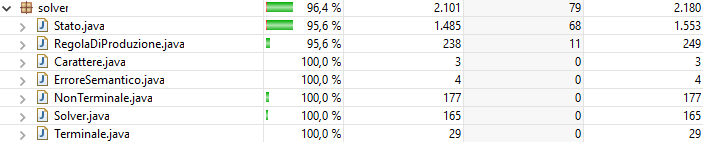
\includegraphics[width=\textwidth]{immagini/SolverCoverage.png}
\caption{Copertura dei test per il package solver}
\end{figure}
\subsubsection{Esiti dei test per la classe Stato}
Per la classe Stato sono stati scritti, all'interno della classe StatoTest, 22 test, superati correttamente dal programma, che garantiscono una copertura della classe Stato pari al $95,6\%$.
\begin{figure}[h]
\centering
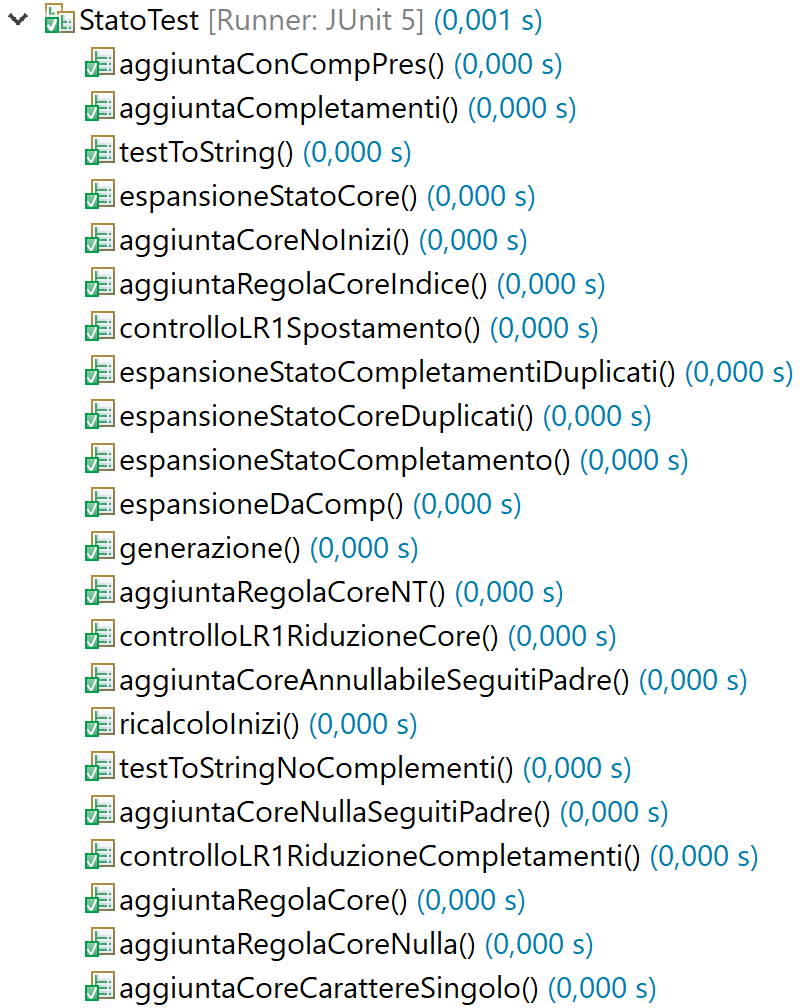
\includegraphics[scale=0.9]{immagini/esitiStatoTest.png}
\caption{Esiti dei test della classe Stato}
\end{figure}
\subsubsection{Esiti dei test per la classe RegolaDiProduzione}
Per la classe RegolaDiProduzione sono stati scritti, all'interno della classe RegolaDiProduzioneTest, 6 test, superati correttamente dal programma, che garantiscono una copertura della classe RegolaDiProduzione pari al $95,6\%$.
\begin{figure}[h]
\centering
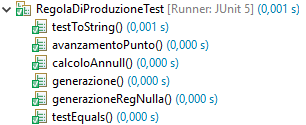
\includegraphics[scale=0.9]{immagini/esitiRegolaDiProduzioneTest.png}
\caption{Esiti dei test della classe RegolaDiProduzione}
\end{figure}
\subsubsection{Esiti dei test per la classe NonTerminale}
Per la classe NonTerminale sono stati scritti, all'interno della classe NonTerminaleTest, 13 test, superati correttamente dal programma, che garantiscono una copertura della classe NonTerminale pari al $100,0\%$.
\begin{figure}[h]
\centering
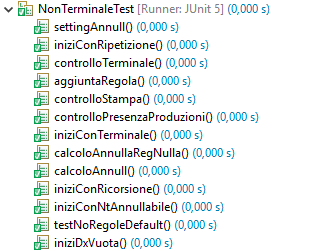
\includegraphics[scale=0.9]{immagini/esitiNonTerminaleTest.png}
\caption{Esiti dei test della classe NonTerminale}
\end{figure}
\pagebreak
\subsubsection{Esiti dei test per la classe Solver}
Per la classe Solver sono stati scritti, all'interno della classe SolverTest, 2 test, superati correttamente dal programma, che garantiscono una copertura della classe Solver pari al $100,0\%$.
\begin{figure}[h]
\centering
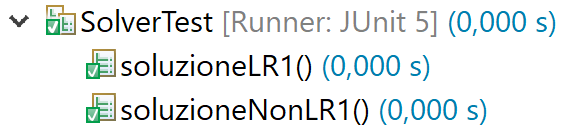
\includegraphics[scale=0.9]{immagini/esitiSolverTest.png}
\caption{Esiti dei test della classe Solver}
\end{figure}
\subsubsection{Esiti dei test per la classe Terminale}
Per la classe Terminale sono stati scritti, all'interno della classe TerminaleTest, 7 test, superati correttamente dal programma, che garantiscono una copertura della classe Terminale pari al $100,0\%$.
\begin{figure}[h]
\centering
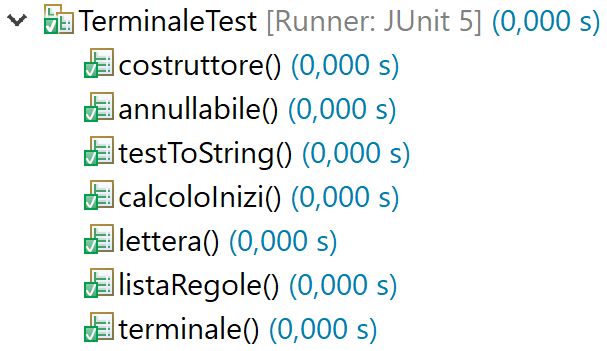
\includegraphics[scale=0.9]{immagini/esitiTerminaleTest.png}
\caption{Esiti dei test della classe Terminale}
\end{figure}
\pagebreak
\subsection{Esiti e copertura dei test di sistema}
I test di sistema sono stati effettuati eseguendo il metodo \textit{main} della classe \textit{Riconoscitore} più volte, passandogli come input i file contenuti all'interno della cartella "lfc$\backslash$resourses" presente nella repository del progetto (\url{https://github.com/d-presciani/progettoLFC}); come oracoli per valutare la correttezza dei test sono stati utilizzati i temi svolti in classe durante il corso di Linguaggi formali e compilatori. \par
Durante i test di sistema è stata rilevata anche la copertura del codice nelle varie esecuzioni; nella seguente immagine è possibile vedere la copertura complessiva (ottenuta combinando la copertura delle singole esecuzioni).
\begin{figure}[h]
\centering
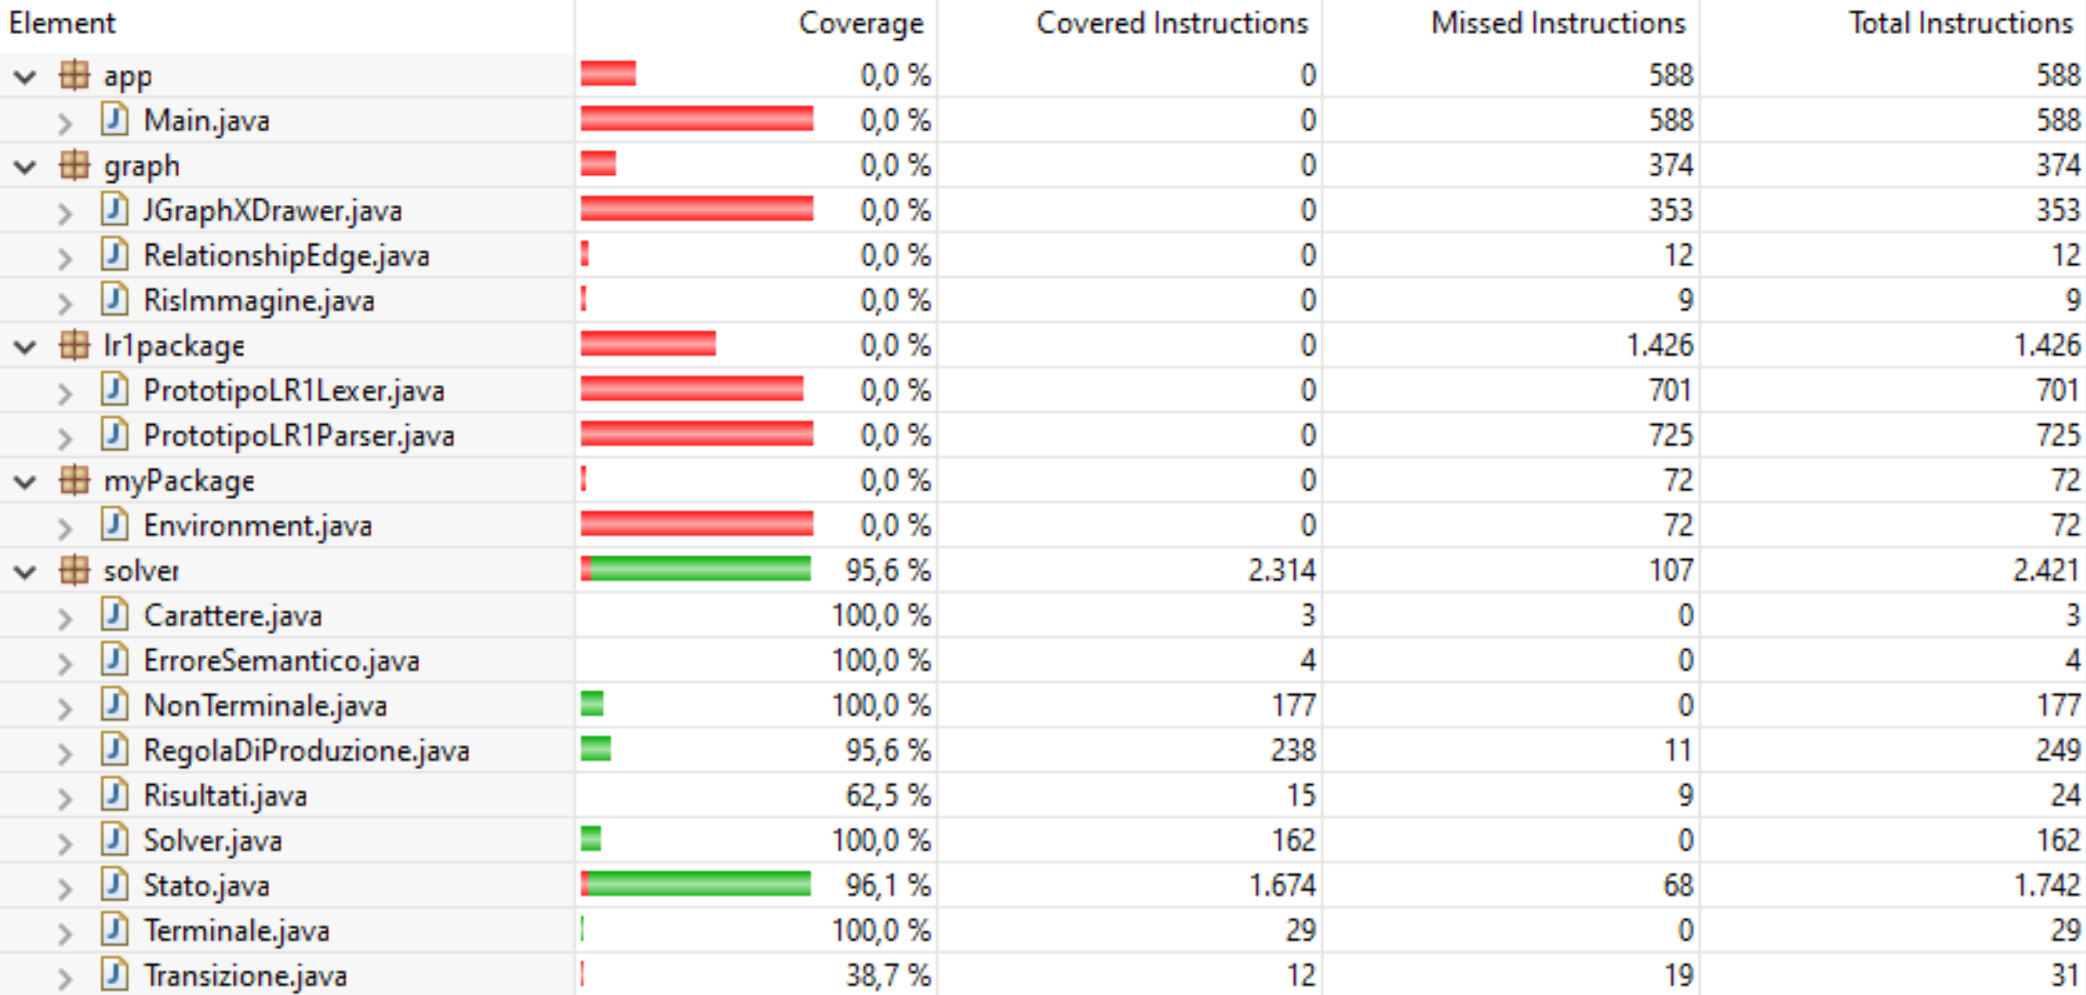
\includegraphics[width=\textwidth]{immagini/codeCoverage.png}
\caption{Copertura del codice relativa ai test di sistema}
\end{figure}
\end{document}